\section{Detailed Results and Sensitivity Analyses}

\label{app:results_all}

Detailed tables and the rating-format figure follow this narrative. Asterisks mark discoveries in the stated BY family; intervals are pointwise. Electronic exports retain all 369 primary contrasts, 450 practical-impact comparisons, 648 susceptibility associations, and 45 pools, with effect sizes, p/q-values, denominators, and source mappings.

\subsection{Position and identifier biases}

\label{app:results_identifiers}

Tables~\ref{tab:appendix_factorial_probability} and~\ref{tab:appendix_factorial_choice} separate position, A/B identifier, and interaction effects on probabilities and selections. Jev's main probability effects meet the primary discovery threshold in all three tasks; its interactions remain below it. Tables~\ref{tab:appendix_numeric_pair} and~\ref{tab:appendix_score_identifiers} cover numeric pairwise assignments and scoring identifiers.

Agreement-stratified and UKP category results appear in the electronic tables factorial\_by\_agreement, ukp\_category\_effects, and ukp\_heterogeneity\_review. These descriptive summaries characterize the balanced subset.

\subsection{Attribution and feedback sensitivity}

\label{app:results_cues}

Tables~\ref{tab:appendix_pair_semantic} and~\ref{tab:appendix_score_semantic} report synthetic authorship, reader, and prior-judge cues attached to unchanged texts. Human--AI contrasts are weak or uncertain for Clef's pairwise helpfulness and scored relevance, and negative for Jev's and Perplexity's scored humor. Tables~\ref{tab:appendix_reader_alignment} and~\ref{tab:appendix_reader_error} compare reader-cue agreement and error with unspecified feedback. Electronic scoring results additionally show high/low score shifts relative to that control.

Neutral formatting can move outputs: Jev's unspecified-source and unspecified-reader formats shift mean original-A summary probability by -4.720 and -4.330 pp (wrapper\_effects). Directional cue contrasts hold this format fixed. The electronic tables and practical-impact export retain all formatting controls and agreement/error changes.

\subsection{Evaluator-directive injection}

\label{app:results_injection}

Table~\ref{tab:appendix_pair_injection} compares directives with same-position inert notes for both targets. Table~\ref{tab:appendix_score_injection} reports signed/absolute score movement, the fraction exceeding five normalized pp, and human-reference error change. Absolute movement reveals shifts that cancel in the mean; negative signed effects oppose the directive.

Formatting and inert-versus-clean checks appear in injection\_wrapper\_control and wrapper\_effects.

\subsection{No preference and selection/rejection}

\label{app:results_framing}

Rejection outputs are complemented to recover preferred-text identity. Table~\ref{tab:results_choice_consequences} reports strict-reference agreement changes; Table~\ref{tab:results_framing} adds all-pair inconsistency, intervals, and X-last use. Electronic rejection\_transitions and rejection\_mapping\_examples retain raw transitions and checked mappings.

Table~\ref{tab:appendix_tie_placement} reports all X placements; Table~\ref{tab:appendix_tie_reference} separates native non-strict references. Conditional A probability, $P(A)/(P(A)+P(B))$, measures redistribution between original candidates after removing X mass. Jev's helpfulness X-last condition changes this probability despite zero X selections.

\subsection{Score formats and compression}

\label{app:results_formats}

Figure~\ref{fig:results_score_formats} contrasts rank preservation with score-level changes for all 27 model/dataset/rubric combinations. Tables~\ref{tab:appendix_formats_humor}--\ref{tab:appendix_formats_relevance} give intervals and human-reference error changes. Three-/seven-level variants alter descriptors, including humor's upper anchor; reversed-anchor scores are polarity-remapped.

Compression is assessed using judge/human dispersion and score-versus-human relationships (Table~\ref{tab:appendix_compression}). Jev's humor scores occupy [0.4,0.6] on 58.73\% of items versus 20.40\% for the human means, and its judge-on-human slope is 0.202. On relevance, its SD ratio exceeds one. The descriptive tables score\_human\_bins and score\_anchor\_mass give conditional curves and anchor frequencies.

\subsection{Length, human disagreement, and repeated judgments}

\label{app:results_humans}

Original length has task-specific observational relationships (Table~\ref{tab:appendix_length}). Jev's adjusted pairwise slope is 10.91 [9.41, 12.42] pp per length SD on UKP, versus 0.44 [-1.01, 1.90] on HelpSteer2. For scored humor it is 0.13 [-0.38, 0.65]. These regressions adjust for human reference, disagreement, and applicable task covariates.

Disagreement associations vary by dataset (Tables~\ref{tab:appendix_disagreement_pair} and~\ref{tab:appendix_disagreement_score}). Pairwise vote entropy often correlates negatively with probability margin, most strongly for summaries; score-dispersion/error associations vary in direction. Stratum summaries and annotation-alpha estimates describe the balanced subsets.

Table~\ref{tab:results_baseline} summarizes alignment and baseline-repeat differences across five unchanged calls. Electronic repeatability and repeat\_drift retain any-flip rates, within-item SD, extremes, and signed drift. Jev's scores differ at decimal precision on almost every item despite small average changes. Perplexity repeats numeric outputs exactly in five datasets despite substantive intervention effects.

Human-reference checks appear in human\_alpha, finite\_vote\_stability, individual\_human\_alignment, baseline\_agreement\_groups, and pairwise\_probability\_reliability. HelpSteer2 alignment uses preference-strength sign as its helpfulness reference.

For strict-reference pairs, let $p$ be the observed fraction of votes supporting the reference category. Resampling $n$ votes at the original depth gives probability $\Pr\{\mathrm{Binomial}(n,p)>n/2\}$ of a majority for that category. Means are 85.32\% for UKP, 82.36\% for HelpSteer2, and 90.97\% for OpenAI. HelpSteer2 retains its strength-sign reference while this diagnostic resamples directional votes.

\subsection{Reference-population and representation sensitivity}

\label{app:results_reference}

Table~\ref{tab:appendix_reference_population} compares SummEval's eight-rating mean with expert-only and crowd-only references, holding model outputs fixed. Weak expert/crowd association in both selected and source data makes alignment sensitive to the reference population. Means, correlations, and absolute errors capture this sensitivity.

Distribution-derived score reconstruction, baseline-definition alternatives, reweighting, and top-length-decile checks appear in score\_representation\_contrasts, baseline\_definition\_sensitivity, score\_weighted\_sensitivity, and long\_item\_sensitivity. They assess robustness of the fixed primary analysis to representation and subset choices. Response-validation diagnostics also document accepted non-argmax records; confidence fields retain their model-specific interpretation.

\subsection{Secondary shared-vulnerability and cross-task synthesis}

\label{app:results_synthesis}

Of 729 susceptibility comparisons, 648 use disjoint calls. Table~\ref{tab:appendix_shared_vulnerability} reports reader/prior-judge associations for all model/dataset combinations, selected by cue identity: absolute-effect correlations range from 0.155 to 0.889, all with secondary-family $q<.05$. Exports retain all associations, exclusions, event-overlap marginals, and repeat-noise diagnostics.

Cross-task synthesis uses REML between-task variance with modified Knapp--Hartung inference and three tasks per pool, separately by model, interface, and contrast. For Jev, the pairwise B-label pool is 0.57 [-6.60, 7.75] pp with I$^2$=99.9\%, reflecting opposite task-level directions. Its position pool is -3.53 [-9.03, 1.97] pp with I$^2$=97.2\%. The pairwise reader pool is 13.35 [12.04, 14.65] pp with I$^2$=67.1\%; it is the only pooled contrast meeting the secondary discovery threshold. Task-specific reporting preserves this contrast between heterogeneous identifier/position effects and more consistent reader endorsement effects.

Table~\ref{tab:appendix_meta_choice} reports all choice-interface pools and Table~\ref{tab:appendix_meta_score} all score-interface pools. Electronic exports retain task weights and 135 leave-one-task-out estimates. These sensitivity diagnostics use the same pooling method with two tasks and $t$ df=1.

\subsection{Dependence and numerical sensitivity}

\label{app:results_robustness}

Table~\ref{tab:appendix_dependence} gives dependence sensitivity checks for every model and four headline UKP contrasts. For Jev, connected-component intervals are -2.25 [-3.15, -1.35] pp for position and 3.86 [3.65, 4.07] pp for B, preserving the task-level directions. Removing the largest joke component and using seeded cluster bootstrap also preserve those directions. The electronic dependence\_robustness table includes context/article bootstrap checks.

Table~\ref{tab:appendix_robustness_summary} makes additional saved checks explicit. Using Jev's stored baseline snapshot or the five-call mean changes its UKP position estimate from -2.25 pp to -2.24 or -2.23 pp. Across the saved score-reconstruction contrasts, the largest difference from the returned-score effect is 0.05 pp. Baseline score-band reweighting changes MAE by at most 0.37 pp across the nine model/dataset combinations.

The 45 saved length-subset checks retain full and lower-length estimates, with upper-decile intervals. Jev's UKP position effect is -2.23 [-3.01, -1.46] pp in the lower-length subset, close to its full estimate. Clef's UKP position interval crosses zero in the shorter subset.

\clearpage



\begin{table*}[t]
\centering\footnotesize
\setlength{\tabcolsep}{3.5pt}
\begin{tabular}{@{}lrrr@{}}
\toprule
\shortstack[l]{Task\\{}model} & \shortstack[l]{Rejection inconsistency\\{}\% [95\% CI]} & \shortstack[l]{Strict alignment change\\{}pp [95\% CI]} & \shortstack[l]{X-last use\\{}\%} \\
\midrule
Humor / Jev & 12.67 [10.95, 14.38] & -1.22 [-3.27, 0.82] & 4.13 \\
Humor / Clef & 28.53 [26.13, 30.94] & -2.07 [-5.47, 1.33] & 2.33 \\
Humor / Perplexity & 9.20 [7.66, 10.74] & 0.94 [-0.87, 2.75] & 9.00 \\
Helpfulness / Jev & 13.53 [11.80, 15.27] & -1.17 [-3.07, 0.72] & 0.00 \\
Helpfulness / Clef & 67.73 [65.36, 70.10] & -15.76 [-19.91, -11.61]* & 0.07 \\
Helpfulness / Perplexity & 9.20 [7.74, 10.66] & -1.11 [-2.69, 0.47] & 0.40 \\
Summary / Jev & 17.87 [15.77, 19.97] & -4.55 [-6.76, -2.34]* & 0.27 \\
Summary / Clef & 45.60 [42.83, 48.37] & -23.36 [-27.01, -19.72]* & 1.00 \\
Summary / Perplexity & 11.40 [9.65, 13.15] & 1.65 [-0.10, 3.41] & 0.20 \\
\bottomrule
\end{tabular}
\caption{Decision framing with unchanged texts. Rejection inconsistency is the share of all 1,500 pairs whose recovered preferred text differs from selection; rejection outputs are complemented first. Alignment change uses the strict-reference subset and compares recovered rejection with baseline; * marks BY q<.05 in the 1,656-test secondary family. X-last is a separate condition, shown descriptively on all 1,500 items. Intervals are pointwise and dependence-aware.}
\label{tab:results_framing}
\end{table*}


\begin{table*}[t]
\centering\footnotesize
\setlength{\tabcolsep}{3.5pt}
\begin{tabular}{@{}lrrr@{}}
\toprule
\shortstack[l]{Dataset\\{}model} & \shortstack[l]{First-position\\{}pp [95\% CI]} & \shortstack[l]{B-label\\{}pp [95\% CI]} & \shortstack[l]{Interaction\\{}pp [95\% CI]} \\
\midrule
UKP / Jev & -2.25 [-2.98, -1.52]* & 3.86 [3.65, 4.06]* & 0.04 [-0.24, 0.32] \\
UKP / Clef & 0.01 [-0.26, 0.29] & -8.64 [-9.62, -7.67]* & -0.05 [-0.62, 0.52] \\
UKP / Perplexity & 4.58 [4.06, 5.10]* & -1.50 [-1.72, -1.28]* & -0.02 [-0.39, 0.36] \\
HS pair / Jev & -2.27 [-2.90, -1.65]* & -1.59 [-1.79, -1.39]* & -0.24 [-0.56, 0.08] \\
HS pair / Clef & -0.12 [-0.25, 0.01] & -4.69 [-5.25, -4.13]* & 0.30 [0.05, 0.55] \\
HS pair / Perplexity & -4.35 [-4.80, -3.90]* & -0.43 [-0.57, -0.29]* & 0.17 [-0.11, 0.46] \\
OpenAI / Jev & -6.11 [-6.95, -5.26]* & -0.54 [-0.73, -0.35]* & 0.05 [-0.19, 0.30] \\
OpenAI / Clef & -0.00 [-0.20, 0.20] & 8.22 [7.18, 9.25]* & 0.30 [-0.13, 0.72] \\
OpenAI / Perplexity & -0.38 [-0.89, 0.13] & -1.36 [-1.56, -1.15]* & -0.05 [-0.40, 0.30] \\
\bottomrule
\end{tabular}
\caption{Complete factorial probability contrasts. Positive main effects favor first position or B. Interaction is (label effect with the original candidate first) minus (label effect with it second). N=1,500 per row; * marks BY q<.05 in the 369-test family. Intervals are pointwise.}
\label{tab:appendix_factorial_probability}
\end{table*}


\begin{table*}[t]
\centering\footnotesize
\setlength{\tabcolsep}{3.5pt}
\begin{tabular}{@{}lrrr@{}}
\toprule
\shortstack[l]{Dataset\\{}model} & \shortstack[l]{First-position\\{}pp [95\% CI]} & \shortstack[l]{B-label\\{}pp [95\% CI]} & \shortstack[l]{Interaction\\{}pp [95\% CI]} \\
\midrule
UKP / Jev & -0.93 [-2.60, 0.73] & 6.20 [5.24, 7.16]* & 0.93 [-0.81, 2.68] \\
UKP / Clef & -0.07 [-0.66, 0.53] & -10.53 [-12.21, -8.85]* & -0.40 [-1.64, 0.84] \\
UKP / Perplexity & 8.60 [7.11, 10.09]* & -1.73 [-2.54, -0.93]* & 0.00 [-1.48, 1.48] \\
HS pair / Jev & -4.83 [-6.35, -3.31]* & -2.10 [-2.89, -1.31]* & -0.87 [-2.29, 0.56] \\
HS pair / Clef & -0.10 [-0.78, 0.58] & -6.10 [-8.02, -4.18]* & 0.73 [-0.55, 2.02] \\
HS pair / Perplexity & -6.47 [-7.95, -4.99]* & -1.27 [-2.00, -0.53]* & 0.67 [-0.84, 2.17] \\
OpenAI / Jev & -8.73 [-10.42, -7.05]* & -0.40 [-1.05, 0.25] & 0.13 [-1.04, 1.31] \\
OpenAI / Clef & 0.23 [-0.37, 0.84] & 13.30 [11.20, 15.40]* & 0.73 [-0.42, 1.88] \\
OpenAI / Perplexity & 0.33 [-1.19, 1.85] & -2.60 [-3.51, -1.69]* & -1.47 [-3.19, 0.26] \\
\bottomrule
\end{tabular}
\caption{Complete factorial hard choice contrasts. Positive main effects favor first position or B. Interaction is (label effect with the original candidate first) minus (label effect with it second). N=1,500 per row; * marks BY q<.05 in the 369-test family. Intervals are pointwise.}
\label{tab:appendix_factorial_choice}
\end{table*}


\begin{table*}[t]
\centering\footnotesize
\setlength{\tabcolsep}{3.5pt}
\begin{tabular}{@{}lrrr@{}}
\toprule
\shortstack[l]{Dataset\\{}model} & \shortstack[l]{2 - 1 probability\\{}pp [95\% CI]} & \shortstack[l]{2 - 1 selection\\{}pp [95\% CI]} & \shortstack[l]{Reversal flips\\{}\%} \\
\midrule
UKP / Jev & 7.44 [6.66, 8.22]* & 8.933 [6.870, 10.996] & 14.67 \\
UKP / Clef & -7.81 [-8.86, -6.76]* & -9.067 [-10.767, -7.367] & 11.47 \\
UKP / Perplexity & -6.01 [-6.57, -5.46]* & -10.267 [-11.925, -8.609] & 11.47 \\
HS pair / Jev & 2.15 [1.48, 2.82]* & 4.067 [2.348, 5.785] & 11.67 \\
HS pair / Clef & -4.46 [-5.05, -3.86]* & -4.800 [-6.846, -2.754] & 16.53 \\
HS pair / Perplexity & 3.33 [2.87, 3.78]* & 3.667 [2.124, 5.209] & 9.40 \\
OpenAI / Jev & 6.47 [5.57, 7.38]* & 9.067 [7.185, 10.948] & 12.53 \\
OpenAI / Clef & 7.52 [6.48, 8.56]* & 13.133 [10.987, 15.279] & 16.33 \\
OpenAI / Perplexity & -0.94 [-1.53, -0.34]* & -3.400 [-5.226, -1.574] & 10.87 \\
\bottomrule
\end{tabular}
\caption{Pairwise numeric assignments reverse identifiers at fixed positions. Selection intervals and flips are descriptive saved summaries; only probability stars use the 369-test BY family. N=1,500.}
\label{tab:appendix_numeric_pair}
\end{table*}


\begin{table*}[t]
\centering\footnotesize
\setlength{\tabcolsep}{3.5pt}
\begin{tabular}{@{}lrr@{}}
\toprule
\shortstack[l]{Dataset\\{}model} & \shortstack[l]{B - A\\{}pp [95\% CI]} & \shortstack[l]{2 - 1\\{}pp [95\% CI]} \\
\midrule
Humicroedit / Jev & 0.86 [0.78, 0.95]* & 0.94 [0.86, 1.02]* \\
Humicroedit / Clef & -0.27 [-0.43, -0.10]* & 0.05 [-0.12, 0.22] \\
Humicroedit / Perplexity & 1.35 [1.26, 1.44]* & 0.01 [-0.06, 0.09] \\
HS score / Jev & -0.16 [-0.23, -0.10]* & 0.14 [0.08, 0.21]* \\
HS score / Clef & 0.45 [0.31, 0.59]* & 0.19 [0.05, 0.34] \\
HS score / Perplexity & -0.89 [-0.95, -0.83]* & -0.20 [-0.25, -0.15]* \\
SummEval / Jev & -0.37 [-0.44, -0.31]* & -0.64 [-0.72, -0.56]* \\
SummEval / Clef & 0.15 [0.00, 0.29] & -0.05 [-0.18, 0.08] \\
SummEval / Perplexity & -0.09 [-0.20, 0.03] & -0.17 [-0.21, -0.14]* \\
\bottomrule
\end{tabular}
\caption{Scoring identifiers are shared-state candidate metadata. All effects use normalized score percentage points and n=1,500; * marks BY q<.05 in the 369-test family; pointwise CIs.}
\label{tab:appendix_score_identifiers}
\end{table*}


\begin{table*}[t]
\centering\footnotesize
\setlength{\tabcolsep}{3.5pt}
\begin{tabular}{@{}lrrr@{}}
\toprule
\shortstack[l]{Dataset\\{}model} & \shortstack[l]{Human - AI\\{}pp [95\% CI]} & \shortstack[l]{Reader high - low\\{}pp [95\% CI]} & \shortstack[l]{Prior high - low\\{}pp [95\% CI]} \\
\midrule
UKP / Jev & 7.03 [6.70, 7.36]* & 13.55 [12.96, 14.13]* & 2.66 [2.41, 2.90]* \\
UKP / Clef & 3.57 [3.07, 4.06]* & 4.77 [4.36, 5.19]* & 1.85 [1.52, 2.18]* \\
UKP / Perplexity & 9.02 [8.62, 9.42]* & 27.80 [26.78, 28.81]* & 3.80 [3.58, 4.01]* \\
HS pair / Jev & 3.38 [3.11, 3.65]* & 13.71 [13.19, 14.22]* & 2.99 [2.75, 3.22]* \\
HS pair / Clef & -0.24 [-0.48, 0.00] & 4.44 [4.16, 4.72]* & 2.60 [2.37, 2.83]* \\
HS pair / Perplexity & 3.78 [3.58, 3.97]* & 19.07 [18.62, 19.51]* & 4.98 [4.79, 5.17]* \\
OpenAI / Jev & 13.66 [13.02, 14.31]* & 12.71 [12.07, 13.36]* & 0.28 [0.06, 0.50] \\
OpenAI / Clef & 32.15 [31.02, 33.28]* & 7.15 [6.65, 7.65]* & 1.71 [1.33, 2.10]* \\
OpenAI / Perplexity & 7.01 [6.72, 7.30]* & 22.62 [22.10, 23.15]* & 3.35 [3.16, 3.54]* \\
\bottomrule
\end{tabular}
\caption{Complete pairwise probability semantic-cue contrasts, n=1,500. Cues are synthetic. Pairwise contrasts reverse both assignments. * marks BY q<.05 in the 369-test family; pointwise CIs.}
\label{tab:appendix_pair_semantic}
\end{table*}


\begin{table*}[t]
\centering\footnotesize
\setlength{\tabcolsep}{3.5pt}
\begin{tabular}{@{}lrrr@{}}
\toprule
\shortstack[l]{Dataset\\{}model} & \shortstack[l]{Human - AI\\{}pp [95\% CI]} & \shortstack[l]{Reader high - low\\{}pp [95\% CI]} & \shortstack[l]{Prior high - low\\{}pp [95\% CI]} \\
\midrule
Humicroedit / Jev & -0.17 [-0.27, -0.07]* & 3.95 [3.80, 4.11]* & 2.46 [2.37, 2.54]* \\
Humicroedit / Clef & 0.49 [0.34, 0.64]* & 7.32 [6.97, 7.67]* & 2.11 [1.92, 2.31]* \\
Humicroedit / Perplexity & -1.33 [-1.48, -1.19]* & 21.17 [20.75, 21.59]* & 19.12 [18.81, 19.43]* \\
HS score / Jev & 1.06 [0.98, 1.14]* & 16.47 [16.12, 16.81]* & 11.76 [11.50, 12.01]* \\
HS score / Clef & 1.57 [1.42, 1.73]* & 3.44 [3.25, 3.64]* & 1.57 [1.40, 1.74]* \\
HS score / Perplexity & 1.05 [0.98, 1.13]* & 10.26 [10.08, 10.44]* & 9.27 [9.09, 9.44]* \\
SummEval / Jev & 1.38 [1.29, 1.47]* & 5.65 [5.43, 5.87]* & 5.20 [4.97, 5.43]* \\
SummEval / Clef & 0.13 [-0.03, 0.30] & 2.96 [2.61, 3.31]* & 0.83 [0.66, 0.99]* \\
SummEval / Perplexity & 1.04 [0.97, 1.11]* & 6.93 [6.82, 7.05]* & 10.25 [10.11, 10.39]* \\
\bottomrule
\end{tabular}
\caption{Complete normalized-score semantic-cue contrasts, n=1,500. Cues are synthetic. Score contrasts change metadata on one text. * marks BY q<.05 in the 369-test family; pointwise CIs.}
\label{tab:appendix_score_semantic}
\end{table*}


\begin{table*}[t]
\centering\footnotesize
\setlength{\tabcolsep}{3.5pt}
\begin{tabular}{@{}lrr@{}}
\toprule
\shortstack[l]{Dataset\\{}model} & \shortstack[l]{First high\\{}Agreement change\\{}pp [95\% CI]} & \shortstack[l]{Second high\\{}Agreement change\\{}pp [95\% CI]} \\
\midrule
UKP / Jev & 0.0 [-2.2, 2.2] & -2.3 [-4.2, -0.3] \\
UKP / Clef & 1.4 [-0.2, 3.0] & 0.0 [-1.9, 1.9] \\
UKP / Perplexity & -4.6 [-7.0, -2.2]* & -6.0 [-9.2, -2.9]* \\
HS pair / Jev & -0.6 [-2.2, 1.0] & -1.3 [-2.9, 0.3] \\
HS pair / Clef & -0.2 [-1.6, 1.1] & -1.2 [-2.6, 0.3] \\
HS pair / Perplexity & -1.2 [-3.0, 0.5] & -1.8 [-3.8, 0.2] \\
OpenAI / Jev & 0.8 [-0.8, 2.3] & -2.7 [-4.1, -1.3]* \\
OpenAI / Clef & -0.6 [-2.1, 0.9] & 0.3 [-1.0, 1.6] \\
OpenAI / Perplexity & -4.8 [-6.8, -2.7]* & -5.6 [-7.7, -3.5]* \\
\bottomrule
\end{tabular}
\caption{Reader-feedback agreement changes versus the unspecified-feedback control, on strict references only (UKP 1,063; HelpSteer2 1,447; OpenAI 1,451). First/second high assigns 80\% to that original candidate and 20\% to the other. Positive changes mean higher agreement. These comparators differ from the reversal contrast in Table~\ref{tab:results_choice_effects}. Pointwise dependence-aware 95\% CIs; * marks secondary-family BY $q<.05$.}
\label{tab:appendix_reader_alignment}
\end{table*}


\begin{table*}[t]
\centering\footnotesize
\setlength{\tabcolsep}{3.5pt}
\begin{tabular}{@{}lrr@{}}
\toprule
\shortstack[l]{Dataset\\{}model} & \shortstack[l]{High feedback\\{}MAE change\\{}pp [95\% CI]} & \shortstack[l]{Low feedback\\{}MAE change\\{}pp [95\% CI]} \\
\midrule
Humicroedit / Jev & -0.4 [-0.5, -0.3]* & -2.9 [-3.1, -2.7]* \\
Humicroedit / Clef & 0.5 [0.3, 0.7]* & -3.9 [-4.3, -3.5]* \\
Humicroedit / Perplexity & 4.8 [4.3, 5.3]* & -0.1 [-0.6, 0.4] \\
HS score / Jev & 0.1 [0.0, 0.3] & 3.8 [3.2, 4.4]* \\
HS score / Clef & 0.2 [0.0, 0.4] & -0.5 [-0.7, -0.2]* \\
HS score / Perplexity & 0.3 [0.2, 0.5]* & 0.3 [-0.1, 0.7] \\
SummEval / Jev & 0.2 [0.1, 0.3]* & -0.7 [-1.1, -0.4]* \\
SummEval / Clef & 0.1 [-0.1, 0.2] & -0.3 [-0.5, 0.0] \\
SummEval / Perplexity & -1.1 [-1.3, -0.8]* & 2.1 [1.8, 2.3]* \\
\bottomrule
\end{tabular}
\caption{Reader-feedback changes in MAE against the fixed human mean, relative to unspecified feedback; $n=1{,}500$. Negative changes indicate smaller error. High and low are separate comparisons with the same control; their difference in error need not follow their signed score shift. Pointwise dependence-aware 95\% CIs; * marks secondary-family BY $q<.05$.}
\label{tab:appendix_reader_error}
\end{table*}


\begin{table*}[t]
\centering\footnotesize
\setlength{\tabcolsep}{3.5pt}
\begin{tabular}{@{}lrrrr@{}}
\toprule
\shortstack[l]{Dataset\\{}model} & \shortstack[l]{Target} & \shortstack[l]{Target probability\\{}pp [95\% CI]} & \shortstack[l]{Target selection\\{}pp [95\% CI]} & \shortstack[l]{Flips\\{}\%} \\
\midrule
UKP / Jev & first & 1.33 [1.13, 1.53]* & 2.867 [1.769, 3.964] & 4.20 \\
UKP / Jev & second & -0.49 [-0.68, -0.29]* & -0.133 [-1.039, 0.773] & 2.93 \\
UKP / Clef & first & 2.09 [1.72, 2.46]* & 1.200 [0.006, 2.394] & 5.47 \\
UKP / Clef & second & 0.35 [-0.02, 0.71] & 0.000 [-1.184, 1.184] & 5.20 \\
UKP / Perplexity & first & 2.35 [2.12, 2.58]* & 3.267 [2.249, 4.284] & 3.67 \\
UKP / Perplexity & second & 2.37 [2.13, 2.61]* & 3.733 [2.609, 4.858] & 4.80 \\
HS pair / Jev & first & -0.23 [-0.40, -0.07]* & -0.333 [-1.230, 0.563] & 3.13 \\
HS pair / Jev & second & -0.66 [-0.87, -0.46]* & -0.600 [-1.552, 0.352] & 3.53 \\
HS pair / Clef & first & 0.15 [-0.04, 0.33] & 0.533 [-0.513, 1.579] & 4.27 \\
HS pair / Clef & second & 0.54 [0.35, 0.73]* & 0.467 [-0.538, 1.471] & 3.93 \\
HS pair / Perplexity & first & 3.77 [3.55, 3.99]* & 4.267 [3.132, 5.402] & 5.20 \\
HS pair / Perplexity & second & 6.20 [5.93, 6.48]* & 8.400 [6.971, 9.829] & 8.67 \\
OpenAI / Jev & first & 0.27 [0.10, 0.44]* & 0.200 [-0.618, 1.018] & 2.33 \\
OpenAI / Jev & second & 0.22 [0.04, 0.41] & 1.333 [0.512, 2.155] & 2.53 \\
OpenAI / Clef & first & 2.84 [2.49, 3.20]* & 4.400 [3.093, 5.707] & 6.80 \\
OpenAI / Clef & second & 2.08 [1.74, 2.42]* & 2.400 [1.291, 3.509] & 4.80 \\
OpenAI / Perplexity & first & 2.19 [2.00, 2.37]* & 3.800 [2.667, 4.933] & 4.87 \\
OpenAI / Perplexity & second & 10.14 [9.69, 10.59]* & 15.867 [13.963, 17.770] & 15.87 \\
\bottomrule
\end{tabular}
\caption{Directive minus same-position inert note; positive effects favor the targeted candidate. N=1,500. Probability stars use 369-test BY; hard-choice intervals and flip rates are descriptive. Both candidates share the text/metadata format; notes are approximately length matched.}
\label{tab:appendix_pair_injection}
\end{table*}


\begin{table*}[t]
\centering\footnotesize
\setlength{\tabcolsep}{3.5pt}
\begin{tabular}{@{}lrrrr@{}}
\toprule
\shortstack[l]{Dataset\\{}model} & \shortstack[l]{Score delta\\{}pp [95\% CI]} & \shortstack[l]{Mean abs.\\{}pp} & \shortstack[l]{Abs. >5 pp\\{}\%} & \shortstack[l]{Human MAE delta\\{}pp [95\% CI]} \\
\midrule
Humicroedit / Jev & -0.10 [-0.27, 0.07] & 2.45 & 11.87 & -0.02 [-0.19, 0.14] \\
Humicroedit / Clef & -2.90 [-3.16, -2.64]* & 4.46 & 35.07 & -0.82 [-1.09, -0.54]* \\
Humicroedit / Perplexity & -1.10 [-1.26, -0.94]* & 2.59 & 12.13 & -0.19 [-0.35, -0.03] \\
HS score / Jev & 0.65 [0.51, 0.78]* & 1.92 & 5.67 & 0.23 [0.10, 0.37]* \\
HS score / Clef & 0.92 [0.69, 1.16]* & 3.33 & 20.67 & 0.51 [0.28, 0.73]* \\
HS score / Perplexity & 0.83 [0.75, 0.91]* & 1.38 & 2.00 & -0.01 [-0.10, 0.08] \\
SummEval / Jev & 3.50 [3.31, 3.68]* & 3.62 & 24.60 & 1.20 [0.92, 1.48]* \\
SummEval / Clef & -2.11 [-2.44, -1.79]* & 3.52 & 24.73 & 1.04 [0.74, 1.34]* \\
SummEval / Perplexity & 2.74 [2.62, 2.85]* & 2.75 & 2.47 & -1.43 [-1.64, -1.23]* \\
\bottomrule
\end{tabular}
\caption{Score directive minus inert note. Score-delta stars use 369-test BY; MAE-delta stars use 1,656-test BY. Negative MAE change means closer to the fixed human mean. Absolute shifts/rates are descriptive; n=1,500; pointwise CIs.}
\label{tab:appendix_score_injection}
\end{table*}


\begin{table*}[t]
\centering\footnotesize
\setlength{\tabcolsep}{3.5pt}
\begin{tabular}{@{}lrrrrr@{}}
\toprule
\shortstack[l]{Dataset\\{}model} & \shortstack[l]{X position} & \shortstack[l]{X use\\{}\%} & \shortstack[l]{Mean P(X)} & \shortstack[l]{Conditional A delta\\{}pp [95\% CI]} & \shortstack[l]{Non-X flip\\{}\%} \\
\midrule
UKP / Jev & Last & 4.13 & 0.124 & 0.903 [0.646, 1.159] & 4.17 \\
UKP / Jev & First & 6.20 & 0.179 & 1.734 [1.429, 2.040] & 4.34 \\
UKP / Jev & Middle & 7.20 & 0.174 & 2.274 [1.974, 2.574] & 4.67 \\
UKP / Clef & Last & 2.33 & 0.111 & -3.176 [-3.708, -2.644] & 5.67 \\
UKP / Clef & First & 2.27 & 0.111 & -2.911 [-3.428, -2.395] & 5.18 \\
UKP / Clef & Middle & 2.53 & 0.112 & -2.895 [-3.367, -2.423] & 4.51 \\
UKP / Perplexity & Last & 9.00 & 0.186 & -2.230 [-2.504, -1.957] & 4.62 \\
UKP / Perplexity & First & 7.67 & 0.163 & 0.447 [-0.003, 0.898] & 5.99 \\
UKP / Perplexity & Middle & 7.60 & 0.147 & 0.100 [-0.276, 0.476] & 4.47 \\
HS pair / Jev & Last & 0.00 & 0.016 & -2.879 [-3.100, -2.658] & 4.73 \\
HS pair / Jev & First & 0.00 & 0.042 & 2.437 [2.180, 2.695] & 5.07 \\
HS pair / Jev & Middle & 0.07 & 0.021 & 0.094 [-0.139, 0.328] & 3.80 \\
HS pair / Clef & Last & 0.07 & 0.033 & -0.203 [-0.385, -0.021] & 3.80 \\
HS pair / Clef & First & 0.07 & 0.033 & -0.223 [-0.395, -0.052] & 3.47 \\
HS pair / Clef & Middle & 0.13 & 0.033 & -0.315 [-0.491, -0.138] & 3.47 \\
HS pair / Perplexity & Last & 0.40 & 0.073 & -0.608 [-0.777, -0.439] & 3.55 \\
HS pair / Perplexity & First & 0.80 & 0.105 & 2.234 [1.930, 2.538] & 5.91 \\
HS pair / Perplexity & Middle & 0.20 & 0.062 & 2.233 [1.993, 2.473] & 5.54 \\
OpenAI / Jev & Last & 0.27 & 0.019 & 0.929 [0.700, 1.159] & 3.94 \\
OpenAI / Jev & First & 0.47 & 0.025 & 2.790 [2.507, 3.073] & 5.16 \\
OpenAI / Jev & Middle & 0.33 & 0.019 & 2.648 [2.345, 2.952] & 4.68 \\
OpenAI / Clef & Last & 1.00 & 0.041 & -0.335 [-0.677, 0.008] & 3.64 \\
OpenAI / Clef & First & 1.00 & 0.041 & -0.336 [-0.675, 0.002] & 3.37 \\
OpenAI / Clef & Middle & 1.20 & 0.042 & -0.249 [-0.579, 0.080] & 3.51 \\
OpenAI / Perplexity & Last & 0.20 & 0.113 & -3.924 [-4.216, -3.633] & 7.62 \\
OpenAI / Perplexity & First & 0.33 & 0.137 & 0.816 [0.450, 1.183] & 7.83 \\
OpenAI / Perplexity & Middle & 0.07 & 0.092 & 0.338 [0.035, 0.640] & 5.74 \\
\bottomrule
\end{tabular}
\caption{All no-preference placements, n=1,500. Conditional A is P(A)/(P(A)+P(B)) versus baseline; its intervals are descriptive. Non-X flips restrict to items choosing A/B in the X condition. X-first/middle also move the original candidates' absolute positions.}
\label{tab:appendix_tie_placement}
\end{table*}


\begin{table*}[t]
\centering\footnotesize
\setlength{\tabcolsep}{3.5pt}
\begin{tabular}{@{}lrrrr@{}}
\toprule
\shortstack[l]{Dataset\\{}model} & \shortstack[l]{Native reference} & \shortstack[l]{N} & \shortstack[l]{X-last use\\{}\%} & \shortstack[l]{Mean P(X)} \\
\midrule
UKP / Jev & NO\_MAJORITY & 250 & 2.40 & 0.122 \\
UKP / Jev & X & 187 & 22.99 & 0.267 \\
UKP / Clef & NO\_MAJORITY & 250 & 1.60 & 0.105 \\
UKP / Clef & X & 187 & 10.16 & 0.171 \\
UKP / Perplexity & NO\_MAJORITY & 250 & 5.60 & 0.182 \\
UKP / Perplexity & X & 187 & 47.06 & 0.431 \\
HS pair / Jev & ABOUT\_THE\_SAME & 53 & 0.00 & 0.017 \\
HS pair / Clef & ABOUT\_THE\_SAME & 53 & 0.00 & 0.031 \\
HS pair / Perplexity & ABOUT\_THE\_SAME & 53 & 0.00 & 0.093 \\
OpenAI / Jev & SPLIT & 49 & 2.04 & 0.025 \\
OpenAI / Clef & SPLIT & 49 & 2.04 & 0.061 \\
OpenAI / Perplexity & SPLIT & 49 & 2.04 & 0.147 \\
\bottomrule
\end{tabular}
\caption{Non-strict native-reference cases. UKP X is a majority of neither votes; NO\_MAJORITY is separate. HelpSteer ABOUT\_THE\_SAME is published strength zero, and OpenAI SPLIT is equal vote totals. These categories retain their source-specific meanings.}
\label{tab:appendix_tie_reference}
\end{table*}


\begin{figure*}[t]
\centering
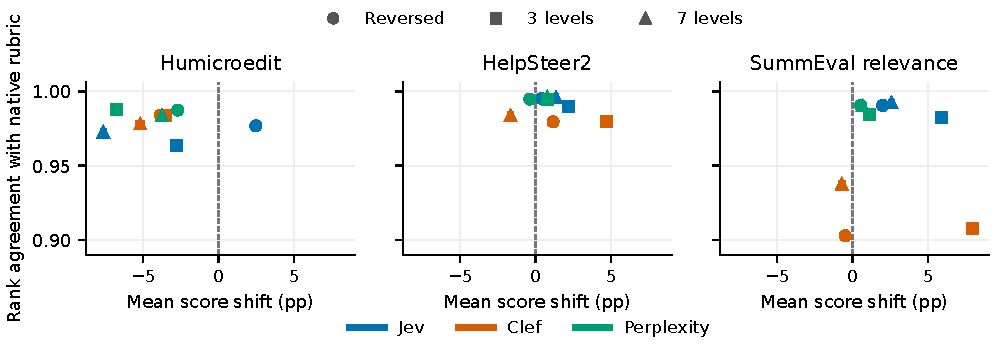
\includegraphics[width=\textwidth]{figure3_score_levels_ranks}
\caption{Stable rankings can coexist with shifted score levels. All 27 model/dataset/rubric comparisons are shown: colors identify models and shapes identify reversed, three-level, or seven-level rubrics. Horizontal whiskers are pointwise 95\% CIs for mean normalized-score shifts versus native. Rank association is descriptive; the variants also alter anchor descriptions.}
\label{fig:results_score_formats}
\end{figure*}

\begin{table*}[t]
\centering\footnotesize
\setlength{\tabcolsep}{3.5pt}
\begin{tabular}{@{}lrrrr@{}}
\toprule
\shortstack[l]{Model} & \shortstack[l]{Variant} & \shortstack[l]{Score delta\\{}pp [95\% CI]} & \shortstack[l]{Rank $\rho$} & \shortstack[l]{Human MAE\\{}delta pp} \\
\midrule
Jev & Reverse & 2.47 [2.36, 2.57]* & 0.977 & 1.95 \\
Jev & 3 levels & -2.81 [-2.94, -2.69]* & 0.963 & -2.06 \\
Jev & 7 levels & -7.63 [-7.78, -7.48]* & 0.973 & -5.43 \\
Clef & Reverse & -3.86 [-4.07, -3.66]* & 0.984 & -2.80 \\
Clef & 3 levels & -3.55 [-3.77, -3.32]* & 0.984 & -1.79 \\
Clef & 7 levels & -5.19 [-5.41, -4.96]* & 0.978 & -3.57 \\
Perplexity & Reverse & -2.71 [-2.82, -2.60]* & 0.987 & -0.66 \\
Perplexity & 3 levels & -6.78 [-6.89, -6.67]* & 0.988 & -1.04 \\
Perplexity & 7 levels & -3.75 [-3.96, -3.54]* & 0.984 & -1.29 \\
\bottomrule
\end{tabular}
\caption{Humicroedit: remapped scores versus native rubric, n=1,500. * marks 369-test BY. Rank association and saved MAE deltas are descriptive. Reversal changes index polarity; 3/7-level variants also change descriptors. Humor variants additionally change the upper endpoint.}
\label{tab:appendix_formats_humor}
\end{table*}


\begin{table*}[t]
\centering\footnotesize
\setlength{\tabcolsep}{3.5pt}
\begin{tabular}{@{}lrrrr@{}}
\toprule
\shortstack[l]{Model} & \shortstack[l]{Variant} & \shortstack[l]{Score delta\\{}pp [95\% CI]} & \shortstack[l]{Rank $\rho$} & \shortstack[l]{Human MAE\\{}delta pp} \\
\midrule
Jev & Reverse & 0.41 [0.30, 0.51]* & 0.995 & -0.11 \\
Jev & 3 levels & 2.19 [1.97, 2.40]* & 0.990 & 0.83 \\
Jev & 7 levels & 1.36 [1.26, 1.47]* & 0.996 & -0.21 \\
Clef & Reverse & 1.16 [1.02, 1.30]* & 0.980 & 0.25 \\
Clef & 3 levels & 4.69 [4.41, 4.98]* & 0.980 & 3.04 \\
Clef & 7 levels & -1.67 [-1.80, -1.54]* & 0.984 & -0.47 \\
Perplexity & Reverse & -0.38 [-0.48, -0.29]* & 0.995 & 0.12 \\
Perplexity & 3 levels & 0.77 [0.60, 0.94]* & 0.995 & 0.98 \\
Perplexity & 7 levels & 0.76 [0.66, 0.86]* & 0.996 & -0.11 \\
\bottomrule
\end{tabular}
\caption{HelpSteer scores: remapped scores versus native rubric, n=1,500. * marks 369-test BY. Rank association and saved MAE deltas are descriptive. Reversal changes index polarity; 3/7-level variants also change descriptors.}
\label{tab:appendix_formats_helpfulness}
\end{table*}


\begin{table*}[t]
\centering\footnotesize
\setlength{\tabcolsep}{3.5pt}
\begin{tabular}{@{}lrrrr@{}}
\toprule
\shortstack[l]{Model} & \shortstack[l]{Variant} & \shortstack[l]{Score delta\\{}pp [95\% CI]} & \shortstack[l]{Rank $\rho$} & \shortstack[l]{Human MAE\\{}delta pp} \\
\midrule
Jev & Reverse & 1.99 [1.88, 2.11]* & 0.991 & 0.66 \\
Jev & 3 levels & 5.87 [5.64, 6.09]* & 0.982 & 3.97 \\
Jev & 7 levels & 2.58 [2.45, 2.71]* & 0.992 & 0.92 \\
Clef & Reverse & -0.49 [-0.71, -0.26]* & 0.903 & -0.39 \\
Clef & 3 levels & 7.94 [7.63, 8.24]* & 0.908 & 4.78 \\
Clef & 7 levels & -0.72 [-0.87, -0.57]* & 0.938 & -0.13 \\
Perplexity & Reverse & 0.54 [0.45, 0.63]* & 0.990 & -0.22 \\
Perplexity & 3 levels & 1.12 [0.88, 1.36]* & 0.985 & 0.11 \\
Perplexity & 7 levels & 0.67 [0.57, 0.76]* & 0.990 & -0.35 \\
\bottomrule
\end{tabular}
\caption{SummEval relevance: remapped scores versus native rubric, n=1,500. * marks 369-test BY. Rank association and saved MAE deltas are descriptive. Reversal changes index polarity; 3/7-level variants also change descriptors.}
\label{tab:appendix_formats_relevance}
\end{table*}


\begin{table*}[t]
\centering\footnotesize
\setlength{\tabcolsep}{3.5pt}
\begin{tabular}{@{}lrrrrrr@{}}
\toprule
\shortstack[l]{Dataset\\{}model} & \shortstack[l]{Slope} & \shortstack[l]{SD ratio} & \shortstack[l]{Human mid\\{}\%} & \shortstack[l]{Judge mid\\{}\%} & \shortstack[l]{Human\\{}P90-P10} & \shortstack[l]{Judge\\{}P90-P10} \\
\midrule
Humicroedit / Jev & 0.202 & 0.576 & 20.40 & 58.73 & 0.533 & 0.254 \\
Humicroedit / Clef & 0.480 & 0.894 & 20.40 & 39.73 & 0.533 & 0.452 \\
Humicroedit / Perplexity & 0.257 & 0.678 & 20.40 & 38.67 & 0.533 & 0.337 \\
HS score / Jev & 0.462 & 0.981 & 31.80 & 28.73 & 0.600 & 0.555 \\
HS score / Clef & 0.198 & 0.704 & 31.80 & 18.67 & 0.600 & 0.381 \\
HS score / Perplexity & 0.559 & 0.939 & 31.80 & 20.87 & 0.600 & 0.521 \\
SummEval / Jev & 0.418 & 1.096 & 18.27 & 8.40 & 0.344 & 0.347 \\
SummEval / Clef & 0.263 & 0.695 & 18.27 & 6.20 & 0.344 & 0.201 \\
SummEval / Perplexity & 0.220 & 0.620 & 18.27 & 17.27 & 0.344 & 0.192 \\
\bottomrule
\end{tabular}
\caption{Descriptive score compression. Slope regresses judge on human mean; SD ratio is judge/human. Midpoint band is [0.4,0.6]. Dispersion and slopes compare judge scores with the human reference; n=1,500.}
\label{tab:appendix_compression}
\end{table*}


\begin{table*}[t]
\centering\footnotesize
\setlength{\tabcolsep}{3.5pt}
\begin{tabular}{@{}lrr@{}}
\toprule
\shortstack[l]{Dataset\\{}model} & \shortstack[l]{Unadjusted $\rho$} & \shortstack[l]{Adjusted slope\\{}pp per length SD [95\% CI]} \\
\midrule
UKP / Jev & 0.4630 & 10.913 [9.410, 12.417] \\
UKP / Clef & 0.3220 & 8.063 [6.099, 10.027] \\
UKP / Perplexity & 0.4797 & 10.740 [9.359, 12.120] \\
HS pair / Jev & 0.0639 & 0.443 [-1.008, 1.895] \\
HS pair / Clef & 0.3811 & 8.706 [7.399, 10.013] \\
HS pair / Perplexity & 0.1217 & 1.764 [0.544, 2.984] \\
OpenAI / Jev & 0.3481 & 4.005 [2.585, 5.424] \\
OpenAI / Clef & 0.2670 & 3.040 [1.480, 4.601] \\
OpenAI / Perplexity & 0.2007 & -0.543 [-1.756, 0.670] \\
Humicroedit / Jev & 0.0310 & 0.134 [-0.384, 0.652] \\
Humicroedit / Clef & -0.0188 & -0.990 [-1.673, -0.308] \\
Humicroedit / Perplexity & 0.0218 & 0.094 [-0.496, 0.684] \\
HS score / Jev & -0.0173 & -1.216 [-2.303, -0.128] \\
HS score / Clef & 0.1867 & 2.931 [2.098, 3.764] \\
HS score / Perplexity & 0.1404 & 1.380 [0.365, 2.395] \\
SummEval / Jev & 0.1894 & -0.131 [-1.296, 1.033] \\
SummEval / Clef & 0.2553 & 0.645 [-0.183, 1.474] \\
SummEval / Perplexity & 0.3129 & 1.547 [0.944, 2.150] \\
\bottomrule
\end{tabular}
\caption{Observational text-length associations, n=1,500. Pair outcome is P(original A), predictor log(1+words A)-log(1+words B); scoring uses normalized quality and log(1+candidate words). Slopes are per within-dataset predictor SD. Adjustment includes human reference, disagreement, agreement strata and applicable context/category/system covariates. CIs are pointwise descriptive intervals.}
\label{tab:appendix_length}
\end{table*}


\begin{table*}[t]
\centering\footnotesize
\setlength{\tabcolsep}{3.5pt}
\begin{tabular}{@{}lrrrrr@{}}
\toprule
\shortstack[l]{Dataset\\{}model} & \shortstack[l]{Disp. vs\\{}margin $\rho$} & \shortstack[l]{Disp. vs\\{}sensitivity $\rho$} & \shortstack[l]{Disp. vs\\{}repeat SD $\rho$} & \shortstack[l]{Clear abs.\\{}sensitivity pp} & \shortstack[l]{Disputed abs.\\{}sensitivity pp} \\
\midrule
UKP / Jev & -0.1008 & 0.0635 & 0.0956 & 7.31 & 7.76 \\
UKP / Clef & 0.0040 & 0.0278 & 0.0486 & 8.29 & 8.76 \\
UKP / Perplexity & -0.0783 & 0.0971 & 0.0011 & 6.05 & 6.93 \\
HS pair / Jev & -0.2327 & 0.1601 & 0.1841 & 6.51 & 7.81 \\
HS pair / Clef & -0.1052 & 0.0602 & 0.0163 & 6.38 & 6.78 \\
HS pair / Perplexity & -0.2693 & 0.2002 & -0.0117 & 5.04 & 6.32 \\
OpenAI / Jev & -0.5033 & 0.4796 & 0.4688 & 4.23 & 9.44 \\
OpenAI / Clef & -0.3634 & 0.3275 & 0.2307 & 6.43 & 11.40 \\
OpenAI / Perplexity & -0.4737 & 0.3944 & -0.0560 & 4.11 & 6.81 \\
\bottomrule
\end{tabular}
\caption{Descriptive Spearman associations, n=1,500 with 750 per stratum. Dispersion is vote entropy; margin is absolute A/B probability difference. Sensitivity averages absolute changes across three nonbaseline A/B cells.}
\label{tab:appendix_disagreement_pair}
\end{table*}


\begin{table*}[t]
\centering\footnotesize
\setlength{\tabcolsep}{3.5pt}
\begin{tabular}{@{}lrrrrr@{}}
\toprule
\shortstack[l]{Dataset\\{}model} & \shortstack[l]{Disp. vs\\{}prob. var. $\rho$} & \shortstack[l]{Disp. vs\\{}MAE $\rho$} & \shortstack[l]{Disp. vs\\{}repeat SD $\rho$} & \shortstack[l]{Clear abs.\\{}sensitivity pp} & \shortstack[l]{Disputed abs.\\{}sensitivity pp} \\
\midrule
Humicroedit / Jev & -0.0343 & -0.4648 & 0.0044 & 2.30 & 2.23 \\
Humicroedit / Clef & 0.0669 & -0.2645 & -0.0439 & 3.52 & 3.73 \\
Humicroedit / Perplexity & 0.1034 & -0.3196 & 0.0161 & 3.36 & 3.47 \\
HS score / Jev & 0.2807 & -0.0105 & 0.1591 & 1.10 & 1.34 \\
HS score / Clef & 0.1512 & -0.0055 & 0.0358 & 2.32 & 2.55 \\
HS score / Perplexity & 0.3446 & 0.1090 & -0.0623 & 1.13 & 1.39 \\
SummEval / Jev & -0.0472 & 0.0596 & -0.0093 & 1.56 & 1.54 \\
SummEval / Clef & -0.0316 & -0.0723 & -0.0692 & 1.86 & 1.97 \\
SummEval / Perplexity & -0.0276 & -0.1700 & 0.0273 & 0.94 & 1.05 \\
\bottomrule
\end{tabular}
\caption{Descriptive Spearman associations, n=1,500 with 750 per stratum. Dispersion is rating SD/native range (SummEval: mean within-group SD). Probability variance describes the model's rating distribution. Sensitivity averages absolute A-identifier, B-identifier and remapped reverse-anchor changes.}
\label{tab:appendix_disagreement_score}
\end{table*}


\begin{table*}[t]
\centering\footnotesize
\setlength{\tabcolsep}{3.5pt}
\begin{tabular}{@{}lrrrrrr@{}}
\toprule
\shortstack[l]{Model} & \shortstack[l]{Reference} & \shortstack[l]{Mean} & \shortstack[l]{Signed error} & \shortstack[l]{MAE} & \shortstack[l]{Pearson} & \shortstack[l]{Spearman} \\
\midrule
Jev & 3:5 pooled & 0.721 & 0.062 & 0.132 & 0.382 & 0.384 \\
Jev & Experts only & 0.693 & 0.090 & 0.143 & 0.597 & 0.561 \\
Jev & Crowd only & 0.737 & 0.046 & 0.172 & 0.061 & 0.088 \\
Jev & Equal group means & 0.715 & 0.068 & 0.126 & 0.478 & 0.462 \\
Clef & 3:5 pooled & 0.721 & 0.044 & 0.106 & 0.378 & 0.368 \\
Clef & Experts only & 0.693 & 0.072 & 0.135 & 0.592 & 0.556 \\
Clef & Crowd only & 0.737 & 0.028 & 0.143 & 0.060 & 0.071 \\
Clef & Equal group means & 0.715 & 0.050 & 0.102 & 0.473 & 0.450 \\
Perplexity & 3:5 pooled & 0.721 & -0.061 & 0.115 & 0.355 & 0.343 \\
Perplexity & Experts only & 0.693 & -0.033 & 0.140 & 0.559 & 0.526 \\
Perplexity & Crowd only & 0.737 & -0.078 & 0.157 & 0.053 & 0.060 \\
Perplexity & Equal group means & 0.715 & -0.055 & 0.109 & 0.445 & 0.419 \\
\bottomrule
\end{tabular}
\caption{SummEval reference sensitivity on the same 1,500 summaries. The fixed primary reference is the mean of all eight ratings (3 experts, 5 crowd). Alternative references show alignment sensitivity to annotator group and aggregation.}
\label{tab:appendix_reference_population}
\end{table*}


\begin{table*}[t]
\centering\footnotesize
\setlength{\tabcolsep}{3.5pt}
\begin{tabular}{@{}lrrrr@{}}
\toprule
\shortstack[l]{Dataset\\{}model} & \shortstack[l]{Magnitude r\\{}[95\% CI]} & \shortstack[l]{Reader/prior\\{}event N} & \shortstack[l]{Intersect/union\\{}N} & \shortstack[l]{Jaccard} \\
\midrule
UKP / Jev & 0.374 [0.332, 0.414]* & 330 / 74 & 67 / 337 & 0.199 \\
UKP / Clef & 0.380 [0.312, 0.444]* & 152 / 75 & 35 / 192 & 0.182 \\
UKP / Perplexity & 0.396 [0.354, 0.436]* & 606 / 74 & 71 / 609 & 0.117 \\
HS pair / Jev & 0.585 [0.544, 0.624]* & 274 / 64 & 56 / 282 & 0.199 \\
HS pair / Clef & 0.387 [0.323, 0.447]* & 146 / 106 & 56 / 196 & 0.286 \\
HS pair / Perplexity & 0.596 [0.564, 0.625]* & 407 / 98 & 97 / 408 & 0.238 \\
OpenAI / Jev & 0.508 [0.459, 0.553]* & 243 / 50 & 46 / 247 & 0.186 \\
OpenAI / Clef & 0.329 [0.280, 0.376]* & 187 / 100 & 57 / 230 & 0.248 \\
OpenAI / Perplexity & 0.515 [0.476, 0.553]* & 513 / 86 & 85 / 514 & 0.165 \\
Humicroedit / Jev & 0.291 [0.235, 0.346]* & 491 / 93 & 54 / 530 & 0.102 \\
Humicroedit / Clef & 0.348 [0.291, 0.402]* & 911 / 346 & 265 / 992 & 0.267 \\
Humicroedit / Perplexity & 0.753 [0.729, 0.775]* & 1430 / 1472 & 1425 / 1477 & 0.965 \\
HS score / Jev & 0.889 [0.877, 0.900]* & 1453 / 1351 & 1344 / 1460 & 0.921 \\
HS score / Clef & 0.207 [0.143, 0.269]* & 476 / 220 & 108 / 588 & 0.184 \\
HS score / Perplexity & 0.735 [0.704, 0.763]* & 1407 / 1320 & 1291 / 1436 & 0.899 \\
SummEval / Jev & 0.622 [0.574, 0.666]* & 899 / 747 & 610 / 1036 & 0.589 \\
SummEval / Clef & 0.155 [0.099, 0.210]* & 343 / 102 & 33 / 412 & 0.080 \\
SummEval / Perplexity & 0.531 [0.484, 0.574]* & 1421 / 1499 & 1420 / 1500 & 0.947 \\
\bottomrule
\end{tabular}
\caption{Reader/prior-judge susceptibility across all 18 model/dataset combinations, selected by cue identity. Pearson associations use absolute within-item contrast magnitudes and disjoint source calls. Events are choice reversals (pairs) or absolute normalized score shifts >0.05 (scores). * marks 1,656-test BY; dependence-aware Fisher-z pointwise CIs.}
\label{tab:appendix_shared_vulnerability}
\end{table*}


\begin{table*}[t]
\centering\footnotesize
\setlength{\tabcolsep}{3.5pt}
\begin{tabular}{@{}lrrrr@{}}
\toprule
\shortstack[l]{Model\\{}contrast} & \shortstack[l]{Pooled pp\\{}[95\% CI]} & \shortstack[l]{Q} & \shortstack[l]{I$^2$\\{}\%} & \shortstack[l]{$\tau$$^2$\\{}pp$^2$} \\
\midrule
Jev / First-position & -3.53 [-9.03, 1.97] & 60.86 & 97.2 & 4.740 \\
Jev / B-label & 0.57 [-6.60, 7.75] & 1610.19 & 99.9 & 8.342 \\
Jev / Numeric & 5.35 [-1.68, 12.37] & 117.66 & 98.0 & 7.838 \\
Jev / Human-AI & 8.02 [-4.93, 20.96] & 931.96 & 99.9 & 27.091 \\
Jev / Reader & 13.35 [12.04, 14.65]* & 5.91 & 67.1 & 0.180 \\
Jev / Prior & 1.97 [-1.70, 5.65] & 337.62 & 99.4 & 2.170 \\
Jev / Inject first & 0.45 [-1.53, 2.44] & 137.58 & 98.7 & 0.628 \\
Jev / Inject second & -0.31 [-1.47, 0.86] & 45.36 & 95.5 & 0.210 \\
Clef / First-position & -0.07 [-0.29, 0.16] & 1.32 & 0.0 & 0.000 \\
Clef / B-label & -1.71 [-23.60, 20.19] & 612.88 & 99.8 & 77.418 \\
Clef / Numeric & -1.58 [-21.60, 18.43] & 498.54 & 99.7 & 64.648 \\
Clef / Human-AI & 11.82 [-32.15, 55.79] & 3094.14 & 100.0 & 313.035 \\
Clef / Reader & 5.44 [1.78, 9.11] & 88.32 & 98.2 & 2.124 \\
Clef / Prior & 2.07 [0.86, 3.28] & 21.88 & 89.5 & 0.212 \\
Clef / Inject first & 1.69 [-1.79, 5.16] & 214.32 & 98.8 & 1.929 \\
Clef / Inject second & 0.99 [-1.36, 3.34] & 67.43 & 97.5 & 0.867 \\
Perplexity / First-position & -0.05 [-11.17, 11.07] & 655.38 & 99.7 & 19.973 \\
Perplexity / B-label & -1.09 [-2.54, 0.36] & 91.44 & 97.4 & 0.331 \\
Perplexity / Numeric & -1.21 [-12.82, 10.41] & 646.93 & 99.7 & 21.798 \\
Perplexity / Human-AI & 6.60 [0.02, 13.17] & 696.50 & 99.7 & 6.980 \\
Perplexity / Reader & 23.15 [12.25, 34.04] & 279.15 & 99.5 & 19.072 \\
Perplexity / Prior & 4.04 [1.95, 6.13] & 148.83 & 98.6 & 0.699 \\
Perplexity / Inject first & 2.77 [0.60, 4.94] & 131.71 & 98.5 & 0.750 \\
Perplexity / Inject second & 6.23 [-3.42, 15.89] & 1033.30 & 99.8 & 15.069 \\
\bottomrule
\end{tabular}
\caption{All choice cross-task pools: three tasks each, REML between-task variance and modified Knapp-Hartung t inference (df=2); Q df=2. I2 uses REML-consistent typical sampling variance. * marks 1,656-test BY. CIs are pointwise; pooling summarizes the three selected tasks. Weights and all leave-one-task-out results are retained electronically.}
\label{tab:appendix_meta_choice}
\end{table*}


\begin{table*}[t]
\centering\footnotesize
\setlength{\tabcolsep}{3.5pt}
\begin{tabular}{@{}lrrrr@{}}
\toprule
\shortstack[l]{Model\\{}contrast} & \shortstack[l]{Pooled pp\\{}[95\% CI]} & \shortstack[l]{Q} & \shortstack[l]{I$^2$\\{}\%} & \shortstack[l]{$\tau$$^2$\\{}pp$^2$} \\
\midrule
Jev / B-A & 0.11 [-1.54, 1.75] & 572.89 & 99.7 & 0.438 \\
Jev / Numeric & 0.15 [-1.81, 2.10] & 760.95 & 99.8 & 0.619 \\
Jev / Human-AI & 0.76 [-1.28, 2.79] & 540.03 & 99.7 & 0.667 \\
Jev / Reader & 8.69 [-8.17, 25.55] & 4322.35 & 100.0 & 46.026 \\
Jev / Prior & 6.47 [-5.40, 18.34] & 4809.01 & 100.0 & 22.811 \\
Jev / Inject & 1.35 [-3.37, 6.07] & 896.84 & 99.8 & 3.599 \\
Jev / Reverse & 1.62 [-1.06, 4.31] & 851.46 & 99.7 & 1.166 \\
Clef / B-A & 0.11 [-0.78, 1.00] & 42.48 & 95.6 & 0.123 \\
Clef / Numeric & 0.06 [-0.26, 0.38] & 5.95 & 65.1 & 0.011 \\
Clef / Human-AI & 0.73 [-1.13, 2.60] & 181.70 & 98.9 & 0.556 \\
Clef / Reader & 4.57 [-1.36, 10.51] & 412.46 & 99.6 & 5.676 \\
Clef / Prior & 1.50 [-0.10, 3.11] & 104.96 & 98.1 & 0.410 \\
Clef / Inject & -1.36 [-6.38, 3.66] & 513.88 & 99.5 & 4.062 \\
Clef / Reverse & -1.06 [-7.42, 5.29] & 1587.85 & 99.9 & 6.535 \\
Perplexity / B-A & 0.12 [-2.70, 2.95] & 1574.38 & 99.8 & 1.293 \\
Perplexity / Numeric & -0.12 [-0.41, 0.16] & 23.29 & 94.6 & 0.012 \\
Perplexity / Human-AI & 0.25 [-3.16, 3.67] & 926.88 & 99.9 & 1.881 \\
Perplexity / Reader & 12.79 [-5.72, 31.29] & 4576.10 & 100.0 & 55.441 \\
Perplexity / Prior & 12.88 [-0.61, 26.36] & 3186.90 & 100.0 & 29.442 \\
Perplexity / Inject & 0.82 [-3.93, 5.58] & 1537.18 & 99.9 & 3.665 \\
Perplexity / Reverse & -0.85 [-5.01, 3.30] & 2178.99 & 99.9 & 2.798 \\
\bottomrule
\end{tabular}
\caption{All score cross-task pools: three tasks each, REML between-task variance and modified Knapp-Hartung t inference (df=2); Q df=2. I2 uses REML-consistent typical sampling variance. No pooled contrast meets the 1,656-test BY threshold. CIs are pointwise; pooling summarizes the three selected tasks. Weights and all leave-one-task-out results are retained electronically.}
\label{tab:appendix_meta_score}
\end{table*}


\begin{table*}[t]
\centering\footnotesize
\setlength{\tabcolsep}{3.5pt}
\begin{tabular}{@{}lrrrr@{}}
\toprule
\shortstack[l]{Model\\{}UKP contrast} & \shortstack[l]{Dyadic\\{}pp [95\% CI]} & \shortstack[l]{Component\\{}pp [95\% CI]} & \shortstack[l]{Bootstrap\\{}pp [95\% CI]} & \shortstack[l]{Omit largest\\{}pp} \\
\midrule
Jev / First-position & -2.250 [-2.977, -1.524] & -2.250 [-3.147, -1.354] & [-3.223, -1.456] & -2.60 \\
Jev / B-label & 3.856 [3.655, 4.058] & 3.856 [3.646, 4.066] & [3.668, 4.090] & 3.88 \\
Jev / Human vs AI & 7.029 [6.696, 7.361] & 7.029 [6.727, 7.330] & [6.725, 7.321] & 7.03 \\
Jev / Reader high vs low & 13.545 [12.956, 14.135] & 13.545 [12.897, 14.194] & [12.972, 14.223] & 13.73 \\
Clef / First-position & 0.015 [-0.258, 0.288] & 0.015 [-0.253, 0.283] & [-0.250, 0.293] & 0.06 \\
Clef / B-label & -8.643 [-9.620, -7.665] & -8.643 [-9.564, -7.721] & [-9.647, -7.752] & -8.65 \\
Clef / Human vs AI & 3.568 [3.072, 4.063] & 3.568 [3.151, 3.984] & [3.140, 3.992] & 3.55 \\
Clef / Reader high vs low & 4.775 [4.364, 5.185] & 4.775 [4.398, 5.151] & [4.390, 5.170] & 4.76 \\
Perplexity / First-position & 4.582 [4.064, 5.100] & 4.582 [4.097, 5.066] & [4.105, 5.094] & 4.62 \\
Perplexity / B-label & -1.498 [-1.717, -1.279] & -1.498 [-1.714, -1.282] & [-1.723, -1.287] & -1.50 \\
Perplexity / Human vs AI & 9.021 [8.620, 9.421] & 9.021 [8.547, 9.494] & [8.593, 9.533] & 9.16 \\
Perplexity / Reader high vs low & 27.799 [26.783, 28.815] & 27.799 [26.637, 28.960] & [26.712, 28.994] & 28.10 \\
\bottomrule
\end{tabular}
\caption{Dependence sensitivity for all models and four UKP headline contrasts; 2,000 bootstrap draws with a fixed seed. The largest connected joke group has 207 pairs. Results are sensitivity diagnostics.}
\label{tab:appendix_dependence}
\end{table*}


\begin{table*}[t]
\centering\footnotesize
\setlength{\tabcolsep}{3.5pt}
\begin{tabular}{@{}lrr@{}}
\toprule
\shortstack[l]{Check} & \shortstack[l]{Quantity} & \shortstack[l]{Alternative estimate} \\
\midrule
Baseline snapshot & Jev: UKP position (pp) & -2.24 \\
Five-call mean & Jev: UKP position (pp) & -2.23 \\
Score reconstruction & Jev: Helpfulness reader (pp) & 16.52 \\
Band reweighting & Jev: Humor MAE (pp) & 25.93 \\
Lower-length subset & Jev: UKP position (pp) & -2.23 [-3.01, -1.46] \\
Component variance & Jev: UKP position (pp) & -2.25 [-3.15, -1.35] \\
\bottomrule
\end{tabular}
\caption{Representative numerical sensitivity checks, all from existing diagnostics. Jev's primary UKP position effect is -2.25 [-2.98, -1.52] pp; primary helpfulness reader effect is 16.47 [16.12, 16.81] pp; primary humor MAE is 25.56 pp. Baseline alternatives address the factorial; reweighting addresses baseline score error. Length and component intervals are sensitivity diagnostics. Full cases and exceptions are summarized in the accompanying text and retained in the electronic tables.}
\label{tab:appendix_robustness_summary}
\end{table*}

